\begin{figure*}[t]
  \centering
  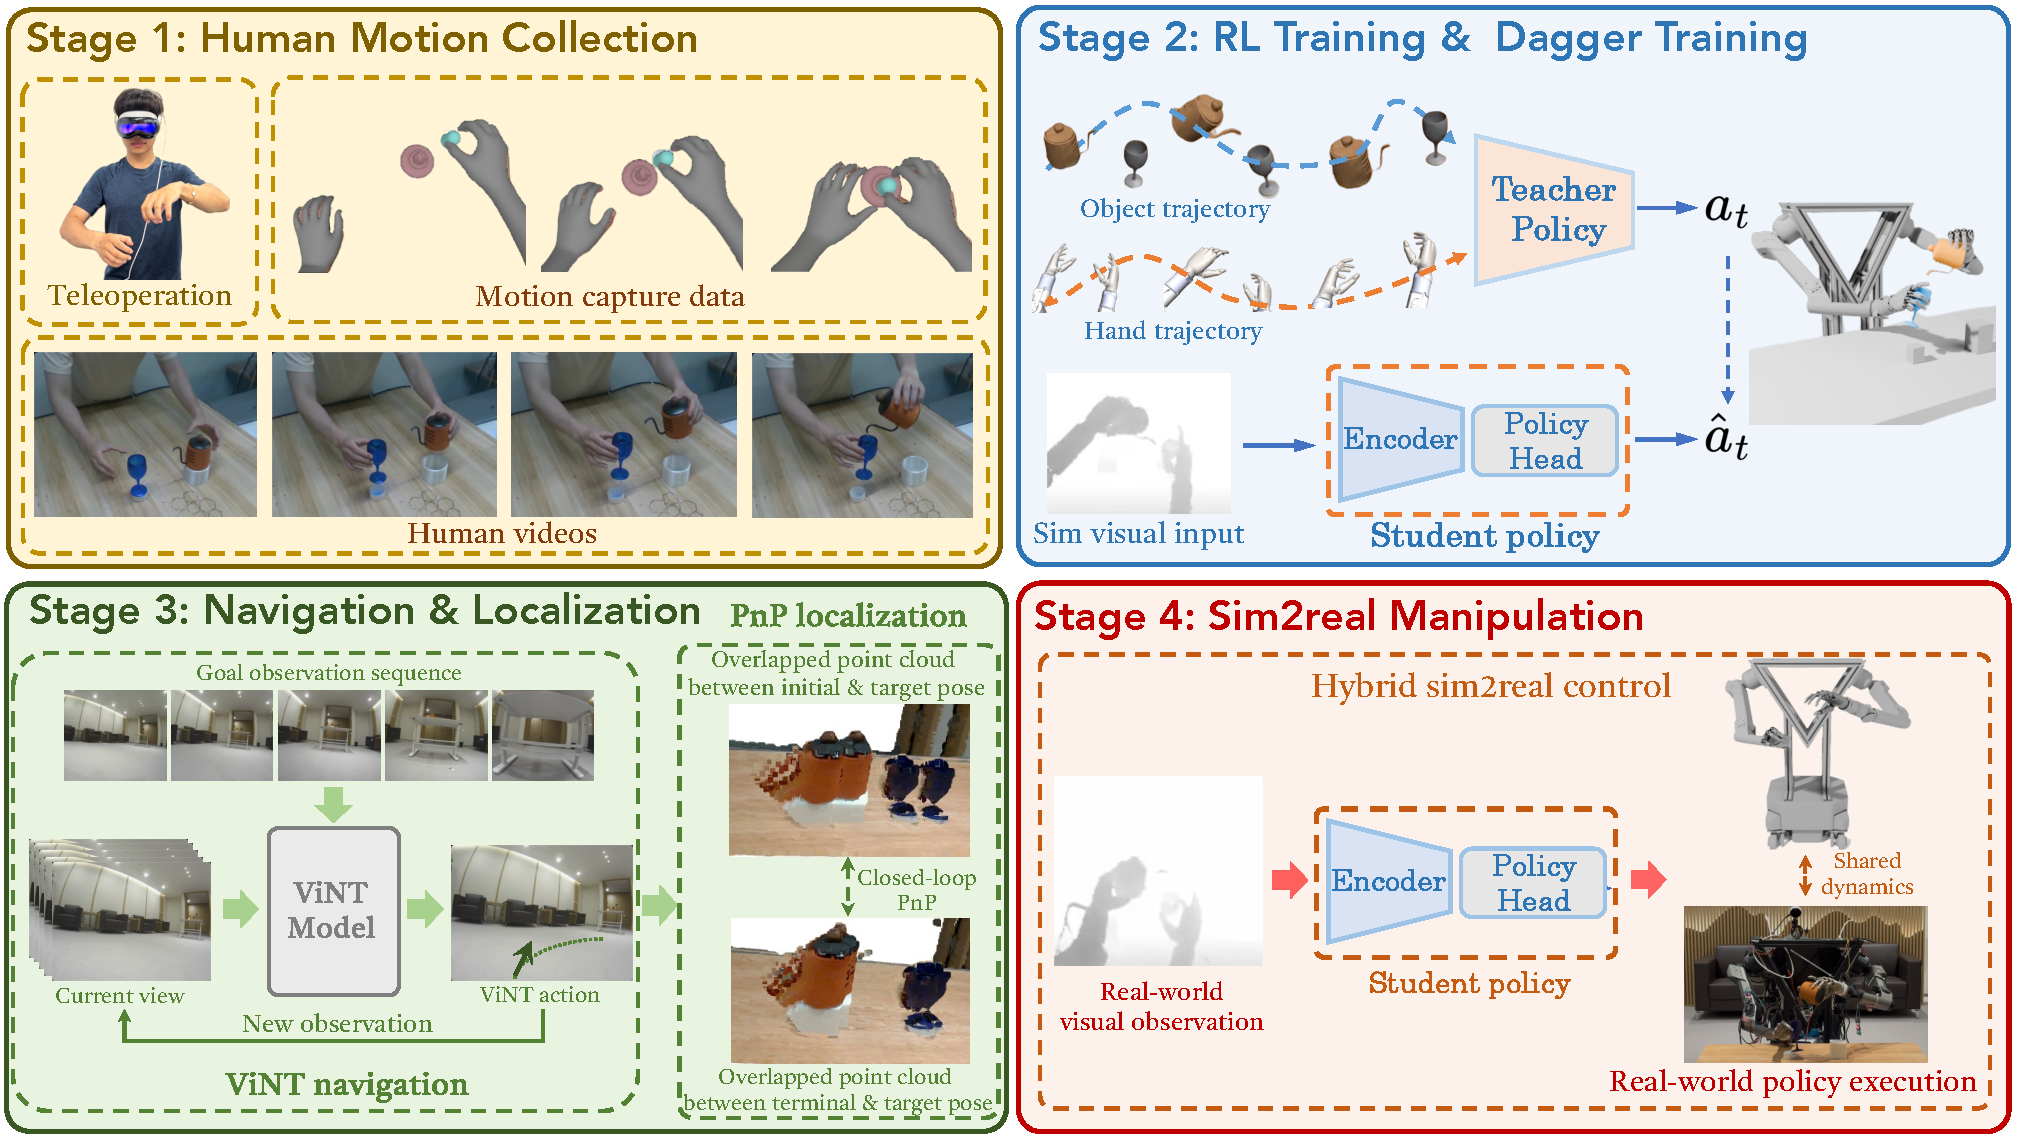
\includegraphics[width=1.0\linewidth]{figures/method_pic.pdf}
  \vspace{-15pt}
  \caption{ \textbf{The main pipeline of \ourshort.} \ourshort comprises a four-stage pipeline for achieving mobile bimanual dexterous manipulation through sim2real transfer. First, we acquire a one‑shot human demonstration drawn from diverse sources. Then, in stage 2, we train a state-based RL teacher policy, then apply DAgger to distill it into a vision‑based student policy. Following this, \ourshort execute long‑horizon navigation using ViNT, followed by closed-loop PnP to finely adjust the robot’s pose and achieve precise alignment in stage 3. Once localization is achieved, the student policy is deployed in a zero‑shot fashion directly in the real world.}
\label{fig:method}
\end{figure*}